\section{ULMFiT}
\begin{frame}[c]{Universal Language Model Fine-tuning for Text Classification}
\begin{itemize}
	\setbeamertemplate{itemize items}[square]
	\item Transfer learning сильно повлияло на компьютерное зрение, но плохо изучено в NLP.
	\item В статье предлагается предобученная модель ULMFiT, которая может быть применена к любой задаче в NLP.
	\item Метод превосходит state-of-the-art результаты на шести задачах классификации текстов.
\end{itemize}
\let\thefootnote\footnote{\href{https://arxiv.org/abs/1801.06146}{\color[rgb]{0.5,0.5,0.5} [Howard et al., 2018]}}
\end{frame}

\begin{frame}[c]{Universal Language Model Fine-tuning for Text Classification}
\begin{figure}
	\centering
	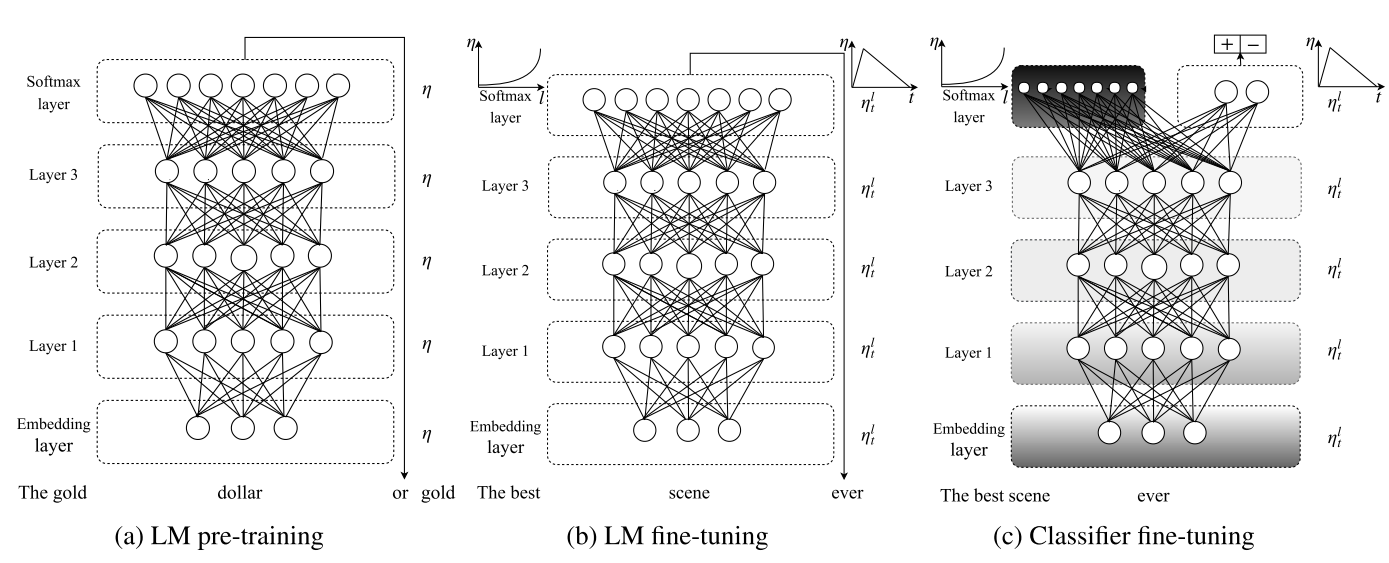
\includegraphics[width=0.8\textwidth]{figures/ulmfit.png}
\end{figure}
\begin{itemize}
	\setbeamertemplate{itemize items}[square]
	\item AWD-LSTM с алгоритмом оптимизации SGD.
	\item Модель предобучается на задаче языковой модели на датасете Wikitext-103 из 103 млн. слов.
	\item Модель дообучается на данных целевой задачи.
	\item Полученная модель дообучается уже на целевой задаче классификации.
\end{itemize}
\end{frame}

\begin{frame}[c]{Universal Language Model Fine-tuning for Text Classification}
\begin{itemize}
	\setbeamertemplate{itemize items}[square]
	\item Slanted triangular learning rates (1cycle):
\end{itemize}
\begin{figure}
	\centering
	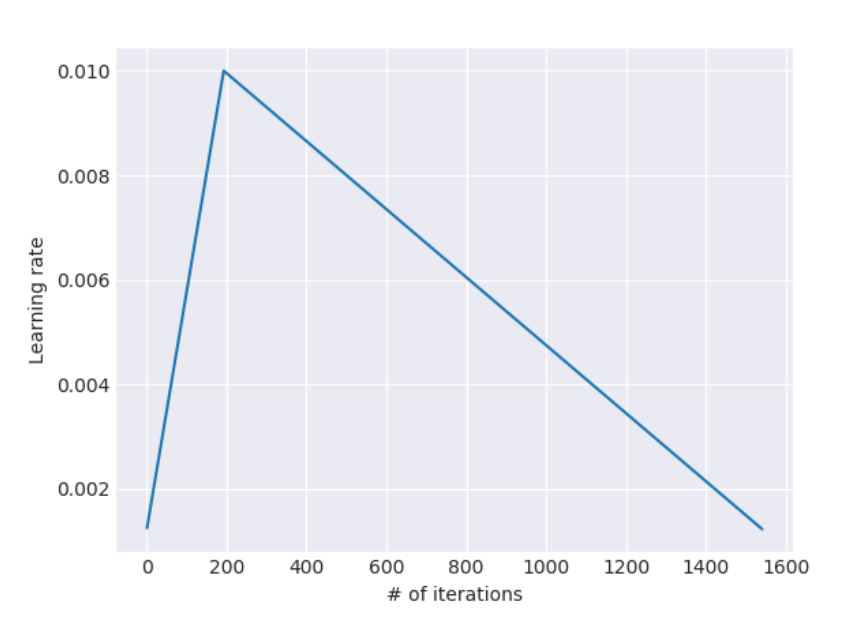
\includegraphics[width=0.7\textwidth]{figures/1cycle.png}
\end{figure}
\end{frame}

\begin{frame}[c]{Universal Language Model Fine-tuning for Text Classification}
\begin{itemize}
	\setbeamertemplate{itemize items}[square]
	\item Discriminative fine-tuning: различные параметры learning rate для различных слоев сети (чем глубже слой, тем больше learning rate).
	\item Concat pooling: для классификации используется не только последнее скрытое состояние $h_T$, а среднее и максимум по всем скрытым состояниям $H = \left\{h_1, . . . , h_T\right\}$:
	\begin{itemize}
		\setbeamertemplate{itemize items}[circle]
		\item $h_c = \left[h_T, maxpool(H), meanpool(H)\right]$;
	\end{itemize}
	\setbeamertemplate{itemize items}[square]
	\item Gradual unfreezing: постепенно размораживаются слои начиная с последнего слоя, поскольку она содержит наименее общие знания и информация.
\end{itemize}
\end{frame}

\begin{frame}[c]{Universal Language Model Fine-tuning for Text Classification}
\begin{itemize}
	\setbeamertemplate{itemize items}[square]
	\item Результаты:
\end{itemize}
\begin{figure}
	\centering
	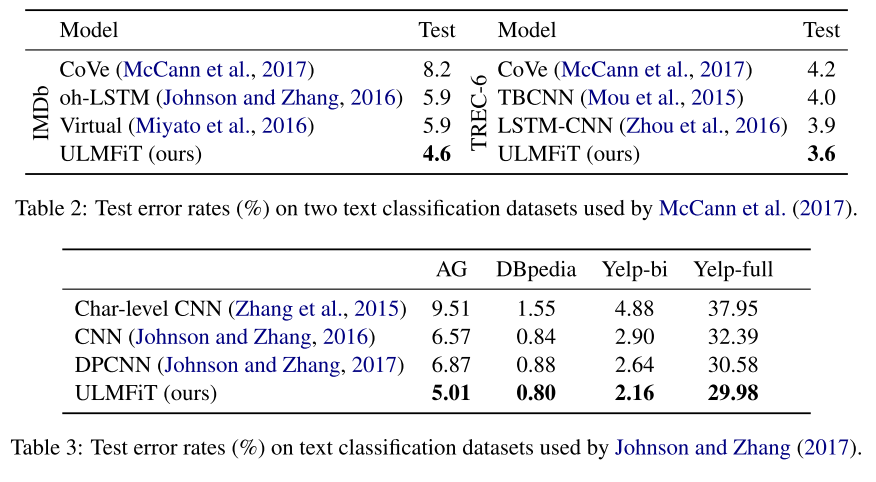
\includegraphics[width=0.9\textwidth]{figures/ulmfitres.png}
\end{figure}
\end{frame}

\begin{frame}[c]{Universal Language Model Fine-tuning for Text Classification}
\begin{itemize}
	\setbeamertemplate{itemize items}[square]
	\item Сравнение предобученной модели с моделью без предобучения:
\end{itemize}
\begin{figure}
	\centering
	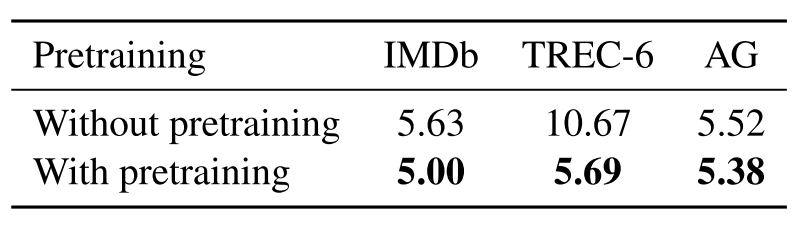
\includegraphics[width=0.9\textwidth]{figures/ulmfit2.png}
\end{figure}
\end{frame}

\begin{frame}[c]{Universal Language Model Fine-tuning for Text Classification}
\begin{itemize}
	\setbeamertemplate{itemize items}[square]
	\item Зависимость ошибки на данных IMDb, TREC-6 и AG (слева направо) от количества данных в обучении:
\end{itemize}
\begin{figure}
	\centering
	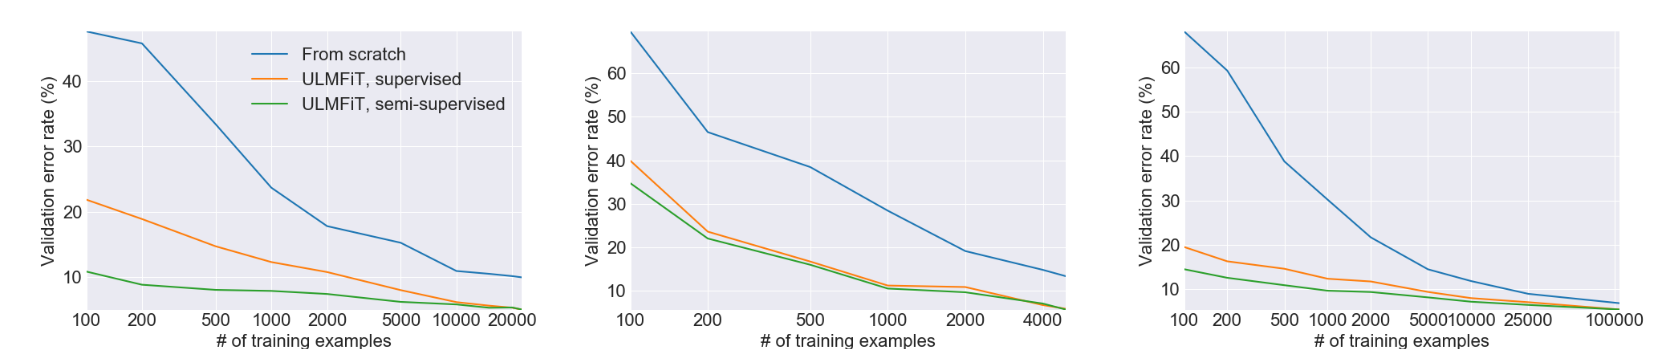
\includegraphics[width=1.0\textwidth]{figures/ulmfitres3.png}
\end{figure}
\end{frame}